\textbf{1.} (3 puntos)


\vspace{20px}
\textit{Solución:}
\\

\begin{enumerate}
[label=\alph*)]
    \item Para estimar la temperatura de la superficie del Sol, consideramos el dato del enunciado que nos dice que su pico de luz
    en el espectro visible se sitúa alrededor del color verde. Por tanto, en la Figura 1 de la radiación del cuerpo negro
    debemos encontrar una curva de temperatura que tenga un máximo en la longitud de onda correspondiente al color verde de la luz visible.\\

    \begin{center}
        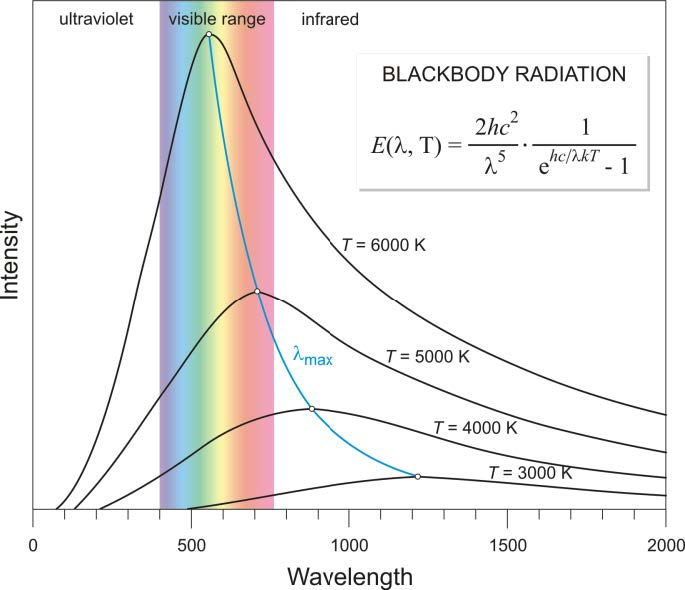
\includegraphics[scale=0.45]{files/img1}
        \captionof{figure}{Radiación del cuerpo negro}
    \end{center}
    \vspace{20px}

    La curva que tiene un pico en esa longitud de onda es $T = 6000K$; por ello, esta es la temperatura
    estimada de la superficie del Sol.

    Se nos ha pedido una estimación de la temperatura, no un cálculo exacto,
    por lo que hemos usado la gráfica de la Figura 1, en vez de
    utilizar la ley de Planck de la radiación del cuerpo negro y el dato de la longitud de onda para el color verde de la luz visible.

    \vspace{20px}
    \item En este caso, no existe una curva de temperatura para $T = 32 500 K$ en la gráfica de la radiación del cuerpo negro.
    Debemos usar entonces la ley de Planck, que describe
    la densidad espectral de la radiación electromagnética que emite un cuerpo negro a una temperatura dada.

    \begin{equation*}
        E(\lambda, T) = \frac{2hc^2}{\lambda^5} \cdot \frac{1}{e^{hc/\lambda k T} - 1}
    \end{equation*}

    Procedemos de la siguiente manera. Derivamos la expresión anterior respecto a la longitud de onda $\lambda$, e igualamos
    la derivada a 0, para encontrar una relación de la temperatura $T$ con la longitud de onda para la que la radiación es
    máxima.

    \begin{align*}
        \frac{\partial E(\lambda, T)}{\partial \lambda}  &= (-5) \cdot \frac{2hc^2}{\lambda^6} \cdot \frac{1}{e^{hc/\lambda k T} - 1}
        + \frac{2hc^2}{\lambda^5} \cdot
        \frac{(-1) e^{hc/\lambda k T} (- \frac{hc}{k T \lambda^2})}{(e^{hc/\lambda k T} - 1)^2} \\
         &= \frac{2hc^2}{\lambda^6} \cdot \frac{1}{e^{hc/\lambda k T} - 1}
        \biggl( -5 + \frac{hc\;e^{hc/\lambda k T}}{\lambda k T  (e^{hc/\lambda k T} - 1)} \biggr) \\
        &= 0
    \end{align*}

    Tras eliminar los términos fuera del paréntesis, nos queda la igualdad:

    \begin{equation*}
        \frac{hc}{\lambda k T} \cdot \frac{e^{hc/\lambda k T}}{e^{hc/\lambda k T} - 1} = 5
    \end{equation*}

    Renombrando $u = \frac{hc}{\lambda k T}$,

    \begin{equation*}
        \frac{u\; e^u}{e^u -1} = 5
    \end{equation*}

    Para resolver esta ecuación, consideramos la función Lambert $W$, que resuelve ecuaciones del tipo ${y\;e^{y}=x}$.
    Si conseguimos expresar nuestra ecuación de esta forma, podemos usar los valores calculados de la función de Lambert
    para obtener nuestro resultado.

    \begin{equation*}
        (u-5)e^{u-5} = -5e^{-5} \hspace{10pt} \Rightarrow \hspace{10pt} u-5 = W(-5e^{-5})
     \end{equation*}

    Deshaciendo el cambio de variable anterior,

    \begin{equation*}
    \frac{hc}{\lambda k T} = 5 + W(-5e^{-5}) \hspace{10pt} \Rightarrow \hspace{10pt}  \lambda = \frac{hc}{kT(5 + W(-5e^{-5}))}
    \end{equation*}

    Ya hemos obtenido la relación que estábamos buscando entre $T$ y $\lambda$ para los picos de radiación. Ahora solo
    nos queda sustituir los valores numéricos para obtener la longitud de onda de la radiación de la estrella del enunciado.
    Para simplificar estos cálculos, utilizamos el siguiente código en Python:\\

    \begin{verbatim}
from scipy.constants import Planck, speed_of_light, Boltzmann
from scipy.special import lambertw
import math

temp = 32500
wavelength = (Planck * speed_of_light /
          (Boltzmann * temp * (5 + lambertw(-5 * math.exp(-5)))))

    \end{verbatim}

    La longitud de onda obtenida es $89.2nm$. Esto sitúa a la radiación de la estrella en el tramo ultravioleta.
    Estudiando la \href{https://astronomy.swin.edu.au/cosmos/H/Harvard+spectral+classification}{clasificación espectral estelar de Harvard},
    nuestra estrella se situaría en la clase O para más de $28.000K$, con color violeta, lo que concuerda con los datos calculados
    anteriormente, ya que el color violeta
    es el que se sitúa más cerca del pico calculado, que recaía sobre la región ultravioleta.

    De todos modos, el color real que se observaría si pudiésemos ver directamente esta estrella, no sería violeta, sino blanco con
    un toque azulado / violeta, ya que la estrella no emitiría radiación solo en este rango. Algo similar sucede
    con el ejemplo del apartado a), ya que aunque el sol tiene su pico de radiación en la zonda verde del espectro de luz visible,
    nosotros no lo vemos de ese color, debido al resto de radiación emitida con otras longitudes de onda.




\end{enumerate}


